\section{Regressão linear}
\begin{frame}{Regressão linear}
 \begin{itemize}
   \item Mínimos quadrados;
   \item Modelo de regressão simples (univariado);
   \begin{itemize}
    \item Formulação;
    \item Premissas.
   \end{itemize}
   \item Distribuição amostral dos estimadores;    
   \item Intervalos de confiança para os coeficientes;
   \item Testes para os coeficientes;
   \item Predição: pontual e intervalar.
   \end{itemize}
\end{frame} 

\begin{frame}{Regressão linear: motivação}
 \begin{figure}
  \begin{center}
   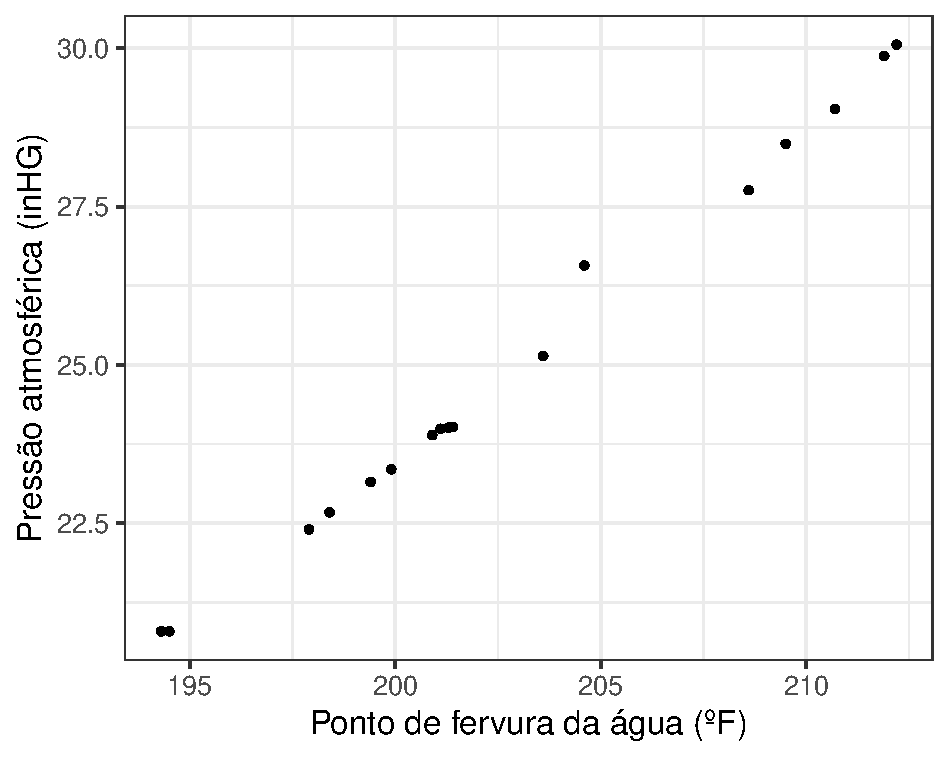
\includegraphics[scale=.6]{figures/pressure_data.pdf}
  \end{center}
 \end{figure}
\end{frame}

\begin{frame}{Mínimos quadrados}
Suponha que estamos interessados na reta 
\begin{equation}
 \label{eq:line}
 y_i = \beta_0  + \beta_1x_i.
\end{equation}
\begin{itemize}
 \item $\beta_0$ é chamado o~\textbf{intercepto} (\textit{intercept}) da reta;
 \item $\beta_1$ é chamado o~\textbf{coeficiente angular} (\textit{slope}) da reta.
\end{itemize}

\begin{theo}[A linha de mínimos quadrados]
\label{thm:least_squares_line}
 Sejam $(x_1, y_1), (x_2, y_2), \ldots, (x_n, y_n)$ uma coleção de $n$ pontos.
 Os valores dos coeficientes que minimizam a soma de quadrados são
 \begin{align*}
  \hat{\beta_0} &= \bar{y} - \hat{\beta_1}\bar{x},\\
  \hat{\beta_1} &= \frac{\sum_{i=1}^n (y_i-\bar{y})(x_i-\bar{x})}{\sum_{i=1}^n \left(x_i - \bar{x}\right)^2},
 \end{align*}
 onde $\bar{x} = (1/n)\sum_{i=1}^n x_i$ e $\bar{y} = (1/n)\sum_{i=1}^n y_i$.
\end{theo}
\textbf{Prova:} Escrever a equação de estimação,$Q = \sum_{i=1}^n \left(y_i - (\beta_0 + \beta_1x_i) \right)^2$, diferenciar $Q$ com respeito aos coeficientes e igualar a zero. 
Ver Teorema 11.1.1 em DeGroot.
\end{frame}

\begin{frame}{O modelo linear}
 Podemos construir um modelo estatístico explícito para a relação entre as variáveis\footnote{Em notação de matrizes,$E[Y] = \bX^T\boldsymbol{\beta}$.} $\bX$ e $Y$:
 \begin{equation}
  \label{eq:lin_mod}
  E[Y \mid \bX = x_1, x_2, \ldots, x_P] = \beta_0 + \beta_1x_1 + \beta_2x_2 + \ldots + \beta_Px_P.  
 \end{equation}
\textbf{Terminologia:}
\begin{itemize}
\item $Y$ é chamada de desfecho,~\textbf{variável-resposta} ou variável dependente;
\item $\bX$ são chamados covariáveis,~\textbf{preditores} ou, ainda, variáveis independentes;
\item $\boldsymbol{\beta} = \{\beta_0, \beta_1, \ldots, \beta_P\}$ são os~\textbf{coeficientes de regressão}.
\end{itemize}

Podemos então idealizar o seguinte modelo
\begin{ideia}[Modelo linear]
 \[ Y_i = \beta_0 + \sum_{j=1}^P \beta_jx_{ij} + \epsilon_i,\: \epsilon_i \sim\operatorname{Normal}(0, \sigma^2).\]
\end{ideia}
\end{frame}

\begin{frame}{Premissas (importante!)}
Como todo modelo, a regressão linear se apoia em premissas sobre os dados e o seu processo gerador.
\begin{itemize}
 \item[P1.] O(s) preditor(es) é (são) conhecido(s);
 \item[P2.] Normalidade: dados os preditores $\bX$, a resposta $Y$ tem distribuição normal;
 \item[P3.] Linearidade na média: a esperança condicional de $Y$ é dada por $\beta_0 + \sum_{j=1}^P \beta_jx_{ij}$;
 \item[P4.] Variância comum (\textbf{homocedasticidade}): a variância condicional de $Y_i$ é  $\sigma^2$ para todo $i = 1, 2, \ldots, n$;
 \item[P5.] Independência (condicional): dados os valores de $\bX$, os valores de $Y$ são idependentes entre si.
\end{itemize}
\end{frame}

\begin{frame}{Cuidado! Quarteto de Anscombe\footnote{Em homenagem ao estatístico Britânico Francis Anscombe (1918-2001).}}
  \begin{figure}
  \begin{center}
   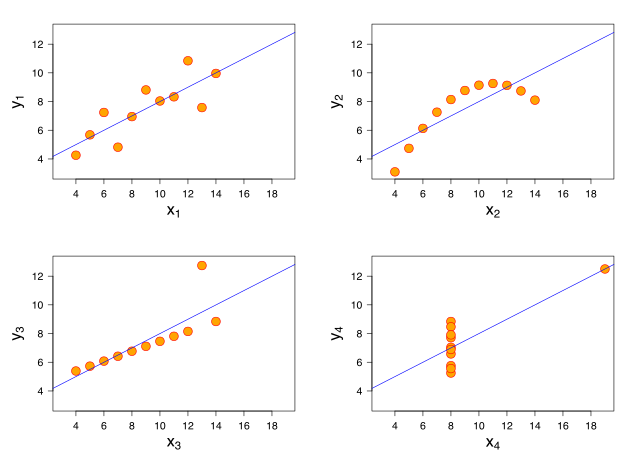
\includegraphics[scale=.435]{figures/anscombe.png}
  \end{center}
  \label{fig:anscombe_quartet}
 \end{figure}
\end{frame}

\begin{frame}{Um teorema interessante}
No modelo linear, a solução de mínimos quadrados e a de máxima verossimilhança coincidem!
\begin{theo}[EMV para os coeficientes de uma regressão linear (simples)]
\label{thm:MLE_linreg_coefficients}
 Sob as premissas já listadas, os estimadores de máxima verossimilhança para $\theta = (\beta_0, \beta_1, \sigma^2)$ são
  \begin{align*}
  \hat{\beta_0}_{\text{EMV}} &= \bar{y} - \hat{\beta_1}_{\text{EMV}}\bar{x},\\
  \hat{\beta_1}_{\text{EMV}} &= \frac{\sum_{i=1}^n (y_i-\bar{y})(x_i-\bar{x})}{\sum_{i=1}^n \left(x_i - \bar{x}\right)^2},\\
  \hat{\sigma^2}_{\text{EMV}} & = \frac{1}{n} \sum_{i=1}^n \left(y_i - (  \hat{\beta_0}_{\text{EMV}} + \hat{\beta_1}_{\text{EMV}} x_i)\right)^2,  
 \end{align*}
 ou seja, os estimadores de máxima verossimilhança dos coeficientes minimizam a soma de quadrados da reta estimada.
\end{theo}
\textbf{Prova:} Ver Teorema 11.2.1 de DeGroot.
\end{frame}

\begin{frame}{Distribuição amostral dos estimadores}
Sob as premissas já discutidas, podemos fazer afirmações sobre a distribuição amostral dos estimadores obtidos:
\begin{theo}[Distribuição amostral dos estimadores dos coeficientes]
\label{thm:sampling_distribution_linreg_coefficients}
   \begin{align*}
  \hat{\beta_0}_{\text{EMV}} &\sim \operatorname{Normal}\left(\beta_0, \sigma^2 \left( \frac{1}{n} + \frac{\bar{x}^2}{s_x^2} \right) \right),\\
  \hat{\beta_1}_{\text{EMV}}  &\sim \operatorname{Normal}\left(\beta_1, \frac{\sigma^2}{s_x^2}\right),\\
  &\operatorname{Cov}\left(\hat{\beta_0}_{\text{EMV}}, \hat{\beta_1}_{\text{EMV}} \right)  = -\frac{\bar{x}\sigma^2}{s_x^2},
 \end{align*}
 onde $s_x = \sqrt{\sum_{i=1}^n (x_i-\bar{x})^2}$.
\end{theo}
\textbf{Prova:} Usar as leis de esperanças e variâncias.
Ver Teorema 11.2.2 de DeGroot.
\end{frame}

\begin{frame}{Intervalos de confiança para os coeficientes}
Podemos computar intervalos de confiança para os coeficientes da regressão linear de maneira muito similar ao que já vimos para o caso da média da Normal.

\begin{theo}[Intervalos de confiança para os coeficientes de uma regressão linear]
\label{thm:CIs_linreg_coefficients}
\begin{align*}
 &\hat{\beta_0} \pm \hat{\sigma}^\prime c\sqrt{\frac{1}{n} + \frac{\bar{x}^2}{s_x^2}}\quad \text{e}\quad \hat{\beta_1} \pm c\frac{\hat{\sigma}^\prime}{s_x},\\
 &\hat{\beta_0} + \hat{\beta_1}x_{\text{pred}} \pm c \hat{\sigma}^\prime \sqrt{\frac{1}{n} + \frac{\left(x_{\text{pred}}-\bar{x}\right)^2}{s_x^2} },
\end{align*}
onde $c = T^{-1}(1-\frac{\alpha_0}{2}; n-2)$ e 
\begin{equation*}
 \hat{\sigma}^\prime := \sqrt{\frac{\sum_{i=1}^n \left(Y_i - \hat{\beta_0} - \hat{\beta_1}x_i \right)^2}{n-2}}.
\end{equation*}
\end{theo}
\textbf{Prova:} Usar o Teorema 11.3.5 de DeGroot e os valores apropriados de $c_0$ e $c_1$.
\end{frame}

\begin{frame}{Testes de hipóteses para o coeficiente angular}
Em geral, estamos interessados em testar a hipótese
\begin{align*}
 H_0 &: \beta_1 = \beta^\star,\\
 H_1 &: \beta_1 \neq \beta^\star.
\end{align*}
Para tanto, podemos computar a estatística
\begin{equation*}
 U_1 = s_x \frac{\hat{\beta_1}-\beta^\star}{\hat{\sigma}^\prime},
\end{equation*}
e computar o p-valor como 
\begin{equation*}
 \pr(U_1 \geq |u_1|) + \pr(U_1 \leq -|u_1|).
\end{equation*}
Notando que $U_1$ tem distribuição t de Student com $n-2$ graus de liberdade sob $H_0$, podemos computar o p-valor exatamente.

Resultados bem similares valem para testar hipóteses sobre $\beta_0$ ou $\hat{Y}$.
\end{frame}

\begin{frame}{Predição pontual}
Suponha que queremos prever o valor de $Y$ para um certo $x_{\text{pred}}$ que não foi observado no experimento.
Podemos compor nossa predição (pountual) como 
\begin{equation}
 \label{eq:lin_pred}
\hat{Y} = \hat{\beta_0} + \hat{\beta_1}x_{\text{pred}}. 
\end{equation}

\begin{theo}[Erro quadrático médio da predição]
\label{thm:MSE_linreg_pred}
 A predição como em~(\ref{eq:lin_pred}) tem erro quadrático médio (EQM) igual a
 \[ E\left[\left(\hat{Y} - Y\right)^2\right] = \sigma^2 \left(1 + \frac{1}{n} + \frac{\left(x_{\text{pred}}-\bar{x}\right)^2}{s_x^2}\right). \] 
\end{theo}
\textbf{Prova:} Ver Teorema 11.2.3 de DeGroot.

\begin{obs}[EQM fora da amostra]
 O EQM aumenta quanto mais longe $x_{\text{pred}}$ estiver dos valores de $X$ que foram medidos (observados).
\end{obs}
\end{frame}

\begin{frame}{Predição intervalar}
Muitas vezes estamos interessados em produzir um~\textit{intervalo} para a nossa predição, ao invés de um único valor (predição pontual). 
Nesta situação, podemos fazer uso do seguinte teorema:
\begin{theo}[Intervalos de \textbf{predição} para $\hat{Y}$]
\label{thm:CI_pred_mean}
A probabilidade de $\hat{Y} = \hat{\beta_0} + \hat{\beta_1}x_{\text{pred}}$ estar no intervalo
\begin{equation*}
 \hat{Y} \pm T^{-1}\left(1-\frac{\alpha_0}{2}; n-2\right)\hat{\sigma}^\prime \sqrt{\left[ 1+ \frac{1}{n} + \frac{\left(x_{\text{pred}}-\bar{x}\right)^2}{s_x^2} \right]},
\end{equation*}
é $1-\alpha_0$.
\end{theo}
\textbf{Prova:} Ver Teorema 11.3.6 de DeGroot.
\end{frame}

\begin{frame}{Intervalos de confiança e de predição: ilustração}
 \begin{figure}
  \begin{center}
   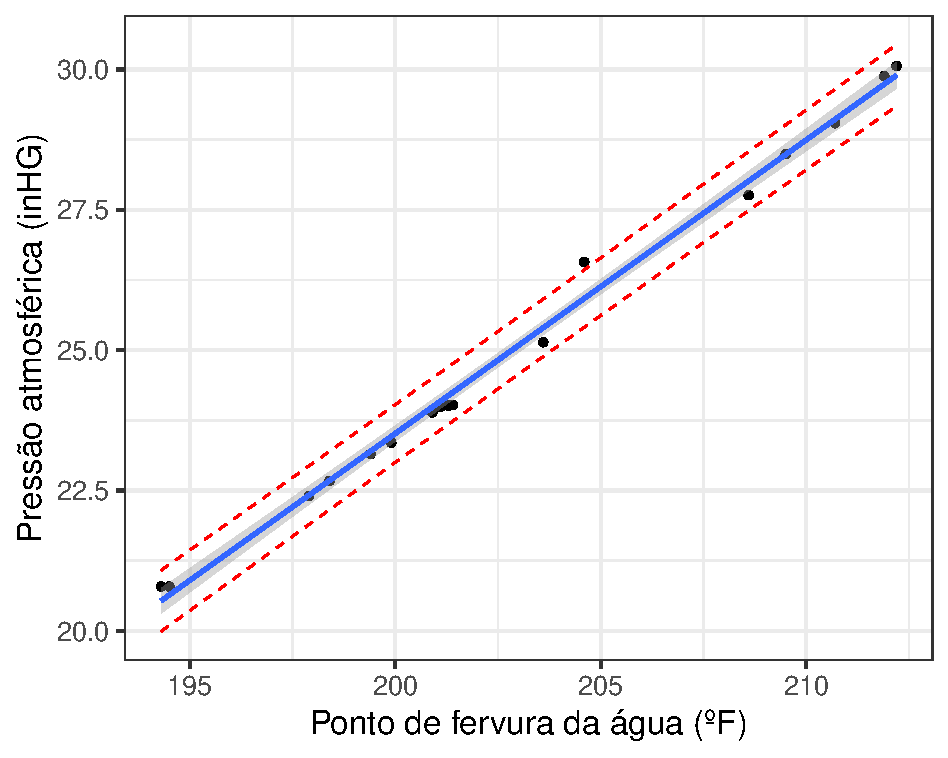
\includegraphics[scale=.6]{figures/pressure_model.pdf}
  \end{center}
 \end{figure}
\end{frame}

\begin{frame}{O que aprendemos?}
\begin{itemize}
  \item[\faLightbulbO] O modelo linear permite modelar a relação (linear) entre uma (ou mais) variável(is) independente(s) e uma variável dependente;    
  \item[\faLightbulbO] A estimação dos coeficientes pode ser feita por mínimos quadrados; 
  \item[\faLightbulbO] A solução de mínimos quadrados é também a solução de máxima verossimilhança!
  \item[\faLightbulbO] Podemos aplicar a teoria Normal para testar hipóteses sobre os coeficientes e calcular intervalos de confiança;
  \item[\faLightbulbO] Podemos produzir predições sobre a variável dependente para valores não-observados da(s) variável(is) independente(s).
   \end{itemize}
 \end{frame} 
 
\begin{frame}{Leitura recomendada}
\begin{itemize}
 \item[\faBook] DeGroot seções 11.1, 11.2 e 11.3;
 \item[\faBook] $^\ast$ Casella \& Berger (2002), seção 11.3.
 \item[\faForward] Próxima aula: DeGroot, seção 9.9;
 \item {\large\textbf{Exercícios recomendados}}
  \begin{itemize}
   \item[\faBookmark] DeGroot, seção 11.1: exercício 3.
   \item[\faBookmark] DeGroot, seção 11.2: exercícios 2, 3 e 6.
   \item[\faBookmark] $^\ast$ Bônus: DeGroot, seção 11.2: exercício  19 (valendo 0.5 na média).
  \end{itemize}
 \end{itemize} 
\end{frame}
